\section{Research Design}

\subsection{Primary quantities}

Let best bid and ask be $b_t$ and $a_t$, with displayed top-level quantities
$q^b_t$ and $q^a_t$. The arithmetic mid and microprice are
\begin{equation}
  m_t=\frac{b_t+a_t}{2}, \qquad
  \mu_t=\frac{q^b_ta_t+q^a_tb_t}{q^b_t+q^a_t}.
\end{equation}
Microprice deviation is $(\mu_t-m_t)/m_t\times10^4$ bps. For horizon $h$,
the population response is forward mid drift,
\begin{equation}
  r_{t,h}=10^4\frac{m_{t+h}-m_t}{m_t}.
\end{equation}

The top-of-book OFI increment follows the event construction in
\citet{cont2014}:
\begin{align}
 e_n={}&\mathbf{1}_{b_n\ge b_{n-1}}q^b_n
       -\mathbf{1}_{b_n\le b_{n-1}}q^b_{n-1} \\
     &-\mathbf{1}_{a_n\le a_{n-1}}q^a_n
       +\mathbf{1}_{a_n\ge a_{n-1}}q^a_{n-1}.
\end{align}
Raw one-second OFI sums $e_n$ over the preceding second. Normalized OFI divides
that sum by mean displayed best-bid-plus-best-ask depth over the contributing
updates. The code definition is in \artifact{src/analysis/ofi_signal.py}.

For a maker fill $i$, let $s_i=+1$ for a buy and $-1$ for a sell. The
fill-conditioned response is
\begin{equation}
  z_{i,h}=10^4s_i\frac{m_{i+h}-m_{i^-}}{m_{i^-}},
\end{equation}
where $m_{i^-}$ is the latest book sample strictly before the fill. This
quantity isolates subsequent mid movement from transaction-price spread
capture. The separate standalone markout diagnostic uses fill price as its
reference and is not substituted into this premise test.

Strictly-pre-fill anchoring is enforced in both the OFI window and reference
mid. A book sample stamped at the fill millisecond is excluded, because it can
already contain the same-millisecond market move associated with the simulated
fill. Tests contain a leakage tripwire for this boundary.

\subsection{Baseline and development panel}

The frozen baseline is a post-only \code{MicropriceMM} on Binance spot
BTCUSDT. It quotes 0.001 BTC on each eligible side, 2 USDT from microprice,
requotes at most every five seconds, and caps position at 0.01 BTC. Historical
execution assumptions are 10 ms entry latency without jitter, a 2 bps maker
fee, a 5 bps taker fee, and queue-cancellation credit evaluated at $c=0$ and
$c=1$. Each nominal five-hour window is the sum of five independently initialized
one-hour replay episodes. Strategy, execution, and inventory state restart each
hour; residual inventory is marked to the session-end mid and then discarded
without a modeled liquidation. The five-hour value is therefore an inference
cluster, not continuous five-hour portfolio P\&L. Latency and fees are modeled
inputs, not measurements from the author's exchange account.

The 2 USDT / five-second baseline was selected during an exploratory April
anchor analysis. Six such anchors were retained among the 24 development
windows. The expanded panel therefore reduces dependence on those examples but
is not an untouched confirmation sample. That qualification is important when
interpreting the later confidence intervals.

\begin{figure}[H]
  \centering
  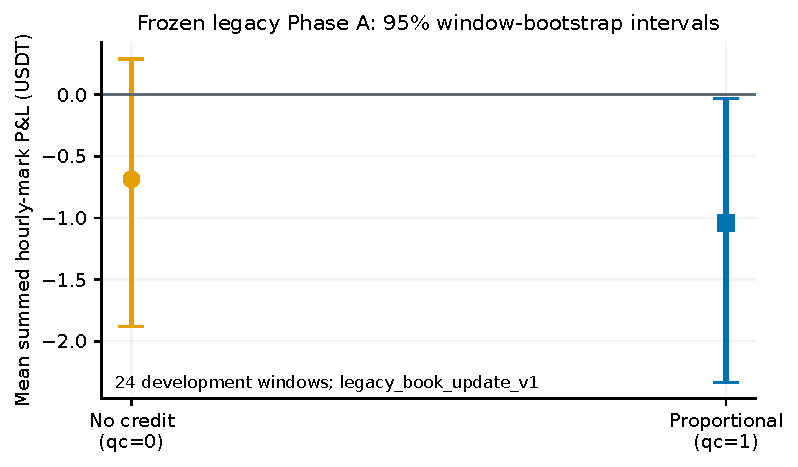
\includegraphics[width=0.78\textwidth]{figures/phase_a_ci.pdf}
  \caption{Phase A estimand: the mean full-strategy net P\&L across 24
  five-hour development windows. Intervals resample windows, not individual
  events.}
  \label{fig:phase-a-ci}
\end{figure}

\subsection{Sequential decision protocol}

The Phase A/B/C sequence and thresholds were written into the repository
before their associated evaluation. This is a pre-specified protocol in the
repository history; it is not an externally registered study.

\begin{enumerate}
  \item \textbf{Phase A---baseline remeasurement.} Estimate mean net P\&L and a
        95\% nonparametric interval by resampling the 24 five-hour windows
        10,000 times with seed 7, separately at $c=0$ and $c=1$.
  \item \textbf{Phase B---premise first.} Before running a strategy that acts
        on OFI, require a stable population association and a material
        fill-conditioned separation. If the premise fails, do not search the
        candidate's thresholds.
  \item \textbf{Phase C---model stress.} Sweep queue-cancellation credit at
        $\{0,.25,.5,.75,1\}$ under 10 ms latency, plus $\{0,50\}$ ms at the two
        credit endpoints. Compare throughput, matched-lot economics, and
        full-strategy P\&L.
\end{enumerate}

The primary one-second normalized-OFI population gate required all of:

\begin{itemize}
  \item one coefficient sign in at least 75\% of development windows;
  \item pooled HAC $|t|\ge2$; and
  \item at least 0.05 bps predicted drift for one signal standard deviation.
\end{itemize}

The conditional gate compared, at 30 seconds, the most-populated negative
side-aligned bucket with the most-populated nonnegative bucket. It required
the latter's mean $z_{i,30s}$ to exceed the former by at least 1.0 bps, with at
least 30 observations in each selected bucket. The 1.0 bps threshold is a
research materiality heuristic and 30 is a minimum-count rule; neither is a
formal power calculation. The chosen comparison also does not test the two
extreme buckets. For those reasons the complete bucket response, its
monotonicity, and its counts must accompany the mechanical gate result.

\subsection{Dependence and uncertainty}

Overlapping forward returns are serially dependent. Pooled regressions
therefore report Newey--West heteroskedasticity-and-autocorrelation-consistent
standard errors \citep{neweywest1987}. The implementation takes the larger of
the overlap-horizon lag count and the Newey--West sample-size rule, capped only
at $n-1$. This corrects standard errors for the specified local dependence
structure, but it does not turn millions of one-second observations into
millions of independent market regimes. The pooled population regression does
not yet carry window-clustered uncertainty across market regimes.

Phase A uncertainty instead resamples whole five-hour windows, preserving
within-window dependence \citep{efron1979}. With only 24 clustered windows,
the interval describes variation within this mechanically selected panel; it
does not estimate sampling variation from a random population of market
regimes. A
future inference pass should add window-clustered uncertainty to both the pooled
population effect and the fill-conditioned bucket contrast rather than
interpreting their raw event counts as independent precision.

\subsection{Holdout discipline}

Twelve late-May windows were selected and their identities hashed alongside
the development panel. This holdout is strategy-sealed rather than unseen. A
pre-strategy regime screen labeled it
\code{regime-shifted}; it had lower realized volatility and fewer jumps than
development. The holdout protocol requires a candidate, parameters, gate
result, and commit to be locked before one evaluation. Because the OFI premise
gate blocked the only candidate, the template remains unlocked and no holdout
strategy output exists. No candidate evaluation was run---there is no favorable
or unfavorable strategy result kept off the page.
